\section{Introduction}
\label{section_intro}
The calculation of planetary orbits is arguably the canonical problem in mathematical physics.
Isaac Newton invented differential calculatus while working on this problem, and used his theory of gravitation to solve it.
In the important special case that one body in the system is a dominant central mass,
and all other bodies are viewed as massless ``test particles'', then a simple closed form solution is possible.
This formulation of the gravitational problem is often called the \href{https://en.wikipedia.org/wiki/Kepler_problem}{Kepler Problem},
named after \href{https://en.wikipedia.org/wiki/Johannes_Kepler}{Johannes Kepler}.
Kepler first studied this problem and published his famous \href{https://en.wikipedia.org/wiki/Kepler\%27s_laws_of_planetary_motion}{three laws of planetary motion},
the first of which states that the planets move in elliptical orbits with the sun at one focus.
This is a surprisingly good approximation for the evolution of the solar system, and the basis for the efficient linearized search over orbital elements developed in this thesis.

The two body approximation is not, however, sufficiently accurate for a high precision model of the past and future positions of the known bodies in the solar system.
While the mass of the sun is much larger than that of the heaviest planet, Jupiter, the planets are sufficiently massive
(and often closer to each other and other bodies of interest) that gravity due to their mass must also be accounted for.
The modern approach to determining orbits in the solar system is to use numerical integrators of the differential equations of motion.

\section{The \tty{REBOUND} Library for Gravitational Integration}
\label{section_rebound}
\tty{REBOUND} is an open source library for numerically integrating objects under the influence of gravity.
It is available on \href{https://github.com/hannorein/rebound}{GitHub}.
It is a first rate piece of software and I would like to thank Matt Holman and Matt Payne for recommending it to me last year.
At the end of Applied Math 225, I wrote a research paper in which I learned to use this library, 
extensively tested it on the solar system, and used it to simulate the near approach of the asteroid Apophis to Earth that will take place in 2029.
In this project, I use \tty{REBOUND} as the ``gold standard'' of numerical integration.
Because of its important role, I describe below how the \tty{IAS15} integrator I selected works.
\footnote{\tty{REBOUND} provides a front end to use multiple integrators. In this project, I make exclusive use of the default \tty{IAS15} integrator.}

The \tty{IAS15} integrator, presented in a 2014 paper by Rein and Spiegel, is a an impressive achievement.
It a fast, adaptive, 15th order integrator for the N-body problem that is (amazingly!) 
accurate to machine precision over a billion orbits.  
The explanation is remarkably simple in comparison to what this algorithm can do.  
Rein and Spiegel start by writing the equation of motion in the form 
$$y'' = F[y', y, t]$$
Here $y$ is the position of a particle; $y'$ and $y''$ are its velocity and acceleration;
and $F$ is a function with the force acting on it over its mass.
In the case of gravitational forces, the only dependence of $F$ is on $y$; 
but one of the major advantages of this framework is its flexibility to support other forces,
including non-conservative forces that may depend on velocity.
Two practical examples are drag forces and radiation pressure.

This expression for $y''$ is expanded to 7th order in $t$, 
$$y''[t] \approx y_0'' + a_0t + a_1t^2 + \cdots +a_6 t^7$$
They next change variables to dimensionless units $h = t / dt$ and coefficients $b_k = a_k dt^{k+1}$:
$$y''[t] \approx y_0'' + b_0h + b_1h^2 + \cdots + b_6 h^7$$
The coefficients $h_i$ represent relative sample points in the interval $[0, 1]$ that subdivide a time step.
Rein and Spiegel call them substeps.  
The formula is rearranged in terms of new coefficients $g_k$ with the property that $g_k$ depends
only on force evaluations at substeps $h_i$ for $i \le k$.
$$y''[t] \approx y_0'' + g_1h + g_2h(h-h_1) + g_3h(h-h_1)(h-h_2) + \cdots + g_8 h (h-h_1) \cdots (h-h_7)$$
Taking the first two $g_i$ as examples and using the notation $y_n'' = y''[h_n]$,
$$g_1 = \frac{y_1'' - y_0''}{h_1} \quad\quad  g_2 = \frac{y_2'' - y_0'' -g_1h_2}{h_2(h_2-h_1)}$$
This idea has a similar feeling to the Jacobi coordinates: a change of coordinates
with a dependency structure to allow sequential computations.

Using the $b_k$ coefficients, it is possible to write polynomial expressions for $y'[h]$ and $y''[h]$:
\begin{align*}
y'[h] &\approx y_0' + h dt \left(y_0'' + \frac{h}{2}\left(b_0 + \frac{2h}{3}\left(b_1 + \frac{}{} \cdots \right)\right) \right) \\
y[h] &\approx y_0 + y_0' h dt + \frac{h^2dt^2}{2}\left(y_0'' + \frac{h}{3}\left(b_0 + \frac{h}{2}\left(b_1 + \frac{}{} \cdots \right)\right) \right)
\end{align*}

The next idea is to use \href{http://mathworld.wolfram.com/RadauQuadrature.html}{Gauss-Radau quadrature}
to approximate this integral with extremely high precision.  
Gauss-Radau quadrature is similar to standard Gauss quadrature for evaluating numerical integrals, 
but the first sample point is at the start of the integration window at $h=0$.
This is a strategic choice here because we already know $y'$ and $y''$ at $h=0$ from the previous time step.
This setup now reduces calculation of a time step to finding good estimate of the coefficients $b_k$.
Computing the $b_k$ requires the forces during the time step at the sample points $h_n$,
which in turn provide estimates for the $g_k$, and then feed back to a new estimate of $b_k$.

This is an implicit system that Rein and Spiegel solve efficiently using what they call a predictor-corrector scheme.
At the cold start, they set all the $b_k=0$, corresponding to constant acceleration over the time step.
This leads to improved estimates of the forces at the substeps, and an improved estimates for the path on the step.
This process is iterated until the positions and velocities have converged to machine precision.
The first two time steps are solved from the cold start this way.  

Afterwards, a much more efficient initial guess is made.  
They keep track of the change between the initial prediction of $b_k$ and its value after convergence,
calling this correction $e_k$.  At each step, the initial guess is $b_k$ at the last step plus $e_k$.
An adaptive criterion is used to test whether the predictor-corrector loop has converged.
The error is estimated as 
$$\widetilde{\delta b_6} = \frac{\max_i |\delta b_{6,i}|}{\max_i |y_i''|}$$
The index $i$ runs over all 3 components of each particle.
The loop terminates when $ \widetilde{\delta b_6} < \epsilon_{\delta b}$; they choose $\epsilon_{\delta b} = 10^{-16}$.
It turns out that the $b_k$ behave well enough for practical problems that this procedure will
typically converge in just 2 iterations!

The stepsize is controlled adaptively with an analogous procedure.
The tolerance is set with a dimensionless parameter $\epsilon_b$,
which they set to $10^{-9}$.
As long as the step size $dt$ is ``reasonable'' in the sense that it can capture
the physical phenomena in question, the error in $y''$ will be bounded by the last term
evaluated at $h=1$, i.e. the error will be bounded by $b_6$.
The relative error in acceleration $\widetilde{b_6} = b_6 / y''$ is estimated as
$$ \widetilde{b_6} = \frac{\max_i |b_{6,i}|}{\max_i |y_i''|}$$
These are similar to the error bounds for convergence of the predictor-corrector loop,
but involve the magnitude of $b_6$ rather than its change $\delta b_6$.
An immediate corollary is that changing the time step by a factor $f$ will change $b_6$
by a factor of $f^7$.

An integration step is computed with a trial step size $dt_{\text{trial}}$.
At the end of the calculation, we compute the error estimate $\widetilde{b_6}$.
If it is below the error tolerance $\epsilon_b$, the time step is accepted.
Otherwise, it is rejected and a new attempt is made with a smaller time step.
Once a time step is accepted, the next  time step is tuned adaptively according to
$dt_{\text{required}} = dt_{\text{trial}} \cdot \left( \epsilon_b / \widetilde{b_6}\right)^{1/7}$
Please note that while the relative error in $y''$ may be of order 7, 
the use of a 15th order integrator implies that 
shrinking the time steps by a factor $\alpha$ will improve the error by a factor of $\alpha^{16}$.

% Hein and Spiegel include an interesting discussion of the different sources of error in N-body integrators.
% They explore the familiar errors arising from the numerical scheme, 
% but also explore both random and biased numerical errors.
% They give a complete error decomposition
% $$E_{\text{tot}} = E_{\text{floor}} + E_{\text{rand}} + E_{\text{bias}} + E_{\text{scheme}}$$
% $E_{\text{floor}}$ is the baseline numerical error that is unavoidable when we try to represent
% real numbers to limited machine precision.
% $E_{\text{rand}}$ is the familiar errors due to accumulated numerical round-off, 
% provided they are distributed randomly (i.e. unbiased).  
% $E_{\text{bias}}$ is an accumulated effect of numerical round-off that has a bias.

% This is a subtle point best illustrated by an example.
% Suppose you have a floating point representation of a 2x2 rotation matrix.
% For a given angle $\phi$, the floating point sum of $\cos^2\phi + \sin^2\phi$
% is likely not to be 1.0 to full machine precision.  
% If it is even a tiny bit less than 1, then repeated application of this rotation matrix
% over many time steps will gradually lead to a contraction.
% Rein and Spiegel devote substantial effort to minimizing rounding errors, 
% particularly by using \href{https://en.wikipedia.org/wiki/Kahan_summation_algorithm}{compensated sums}.
% This simple idea adds only slightly to the run time but can lead to significant accuracy improvements,
% especially over long term simulation, e.g. on the order of one billion orbital periods.

% Rein and Spiegel test the phase accuracy of \tty{IAS15} by running integrating the 
% outer solar system forward in time for 50 orbits with a fixed time step,
% then backwards for 50 orbits with the same time step.
% The known answer is that the phases should be the same, allowing for sharp accuracy measurements.
% This test shows that \tty{IAS15} is more accurate than the comparisons including WH at preserving phases.

% They also introduce a criterion of optimality and demonstrate that \tty{IAS15} integrator satisfies it.
% A result called Brouwer's Law status that in the presence of round-off, 
% a cumulative sum will have have an error that scales as $n^{1/2}$, i.e. it is a random walk of $n$ steps.
% Angular type variables including the orbital phase grow as $n^{3/2}$.
% The authors tested \tty{IAS15} and other integrators on a long term integration of the outer solar system
% (Jupiter, Saturn, Uranus, Neptune) for one billion Jupiter orbits, approximately 12 billion years.
% The energy errors satisfied Brouwer's law, and grew more slowly than those made by the other schemes.
% One surprising conclusions is that the non-symplectic \tty{IAS15} integrator is ``more symplectic''
% (in the sense of having smaller energy errors) than the symplectic integrators!
% This is a completely non-obvious results, and shows the importance of analyzing and understanding
% all the sources of error in a calculation.

\section{A Brief Review of the Keplerian Orbital Elements}
\label{section_orbital_elements}
In his work on the two body problem and the orbits of the planets, Kepler defined six 
\href{https://en.wikipedia.org/wiki/Orbital_elements}{orbital elements}
that are still in use today.
A set of orbital elements pertains to a body as of a particular instant in time, which is typically referred to as the ``epoch'' in this context.
The data sources I've seen all describe the time as a floating point number in the \href{https://en.wikipedia.org/wiki/Julian_day}{Modified Julian Day} (mjd) format.
In particular, I obtained orbital elements for all the known asteroids from \href{https://ssd.jpl.nasa.gov/?sb_elem}{JPL small body orbital elements}
as of MJD 58600, corresponding to 27-Apr-2019 on the Gregorian calendar.\\
Here is a brief review of the definitions of these orbital elements

\begin{figure}
\begin{center}
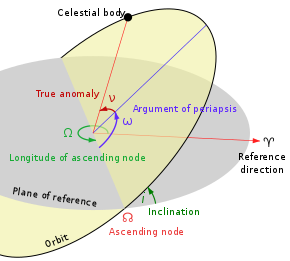
\includegraphics[width=0.40\textwidth]{orbital-elements-wikipedia.png}
\caption{Definition of the traditional Keplerian
\href{https://en.wikipedia.org/wiki/Orbital_elements}{orbital elements}
orbital elements, courtesy of Wikipedia.\\
Two parameters define the shape and size of the ellipse;
two define the orientation of the orbital plane; 
and the last two orient the ellipse in its plane and the phase of the body on its ellipse.}
\end{center}
\end{figure}

\begin{samepage}
\begin{itemize}
\item $a$, the semi-major axis; named \tty{a} in JPL and REBOUND
\item $e$, the eccentricity; named \tty{e} in both systems
\item $i$, the inclination; named \tty{i} in JPL and \tty{inc} in REBOUND
\item $\Omega$, the longitude of the ascending node; named \tty{node} in JPL and \tty{Omega} in REBOUND
\item $\omega$, the argument of perihelion; named \tty{peri} in JPL and \tty{omega} in REBOUND
\item $f$, the true anomaly; named \tty{f} in REBOUND; not quoted directly by JPL
\item $M$, the mean anomaly; named \tty{M} in both systems
\item mjd, the epoch as a Modified Julian Date
\end{itemize}
\end{samepage}
Distances are in A.U. in both JPL and REBOUND.  \\
Angles are quoted in degrees in JPL and in radians in REBOUND.

These orbital elements have stood the test of time because they are useful and intuitive.
They are ideal for computations, both theoretical and numerical, because in the case of the two body problem five of the six orbital elements remain constant.
The careful reader will note that there are 8 entries in the table above, but I've described elements as coming six at a time.
The epoch is considered to be the ``seventh element'' because in the Kepler two body problem, we can describe one body at different times, but it will have the same orbit.
This point of view extends to the N-body problem, which is fully reversible; the same system can be described at at different moments in time.
In practice, the orbital elements are often used to describe the initial conditions of all the bodies for an integration.
The problem is then integrated numerically, possibly both forwards and backwards.
Orbital elements can be reported for any body of interest.

A body orbiting the sun has six degrees of freedom.  
In Cartesian coordinates, there are three for the position and three for the velocity.
In orbital elements, the first five are almost always $(a, e, i, \Omega, \omega)$.
These five will remain constant for a body moving in the Kepler two body problem.

There is some variation in the choice of the sixth element, because different representations have different pros and cons.
The true anomaly $f$ is most convenient for transforming back and forth between orbital elements and Cartesian space.
The mean anomaly $M$ is most convenient for studying the time evolution of the system, because it changes linearly with time in the Kepler two body problem.
The mean anomaly and true anomaly are related by the famous 
\href{https://en.wikipedia.org/wiki/Kepler\%27s_equation}{Kepler's Equation}
This relates the mean anomaly $M$ to the eccentric anomaly $E$.
The \href{https://en.wikipedia.org/wiki/Eccentric_anomaly}{eccentric anomaly} is yet another angle describing a body in orbit.
\begin{figure}
\begin{center}
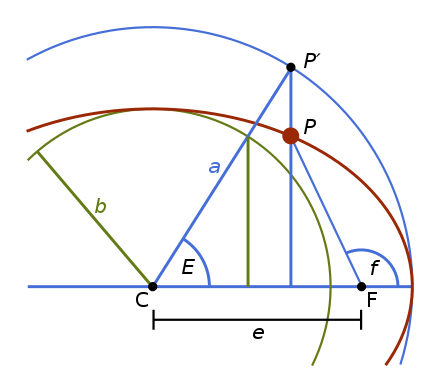
\includegraphics[width=0.40\textwidth]{orbital-anomalies.png}
\caption{Three Orbital Anomalies: Eccentric, Mean and True}
\end{center}
\end{figure}

\begin{align*}
\tan \left(\frac{f}{2} \right) &= \sqrt{\frac{1+e}{1-e}} \tan \left( \frac{E}{2} \right) \\
M &= E - e \sin(E)
\end{align*}
 
The linear evoluation of the mean anomaly, along with Kepler's equation, allows us to efficiently compute orbits for the Kepler two body problem.
The relationship between the eccentric anomaly $E$ and true anomaly $f$ is a one to one function that can be evaluated fast on a computer.
The mapping from eccentric anomaly $E$ to mean anomaly $M$ is also fast.
The inverse mapping from $M$ to $E$ does not have a known analytical form.
But it can be evaluated raplidly using Newton's Method with a reasonable initial guess.
This is the method that I use to compute the orbits under the Kepler approximation. 

\section{Numerical Integration of the Planets and Asteroids}
\label{section_numerical_integration}

I have described above a library \tty{REBOUND} that can efficiently integrate the solar system,
and a data source Horizons that can be used to obtain accurate initial conditions for solar bodies.
In principle integrating the solar system is a straightfoward exercise.
In practice, there are quite a few details that need to be worked out before you can obtain reliably correct answers.
You need to carefully specify the bodies you submit to Horizons.
Horizons has separate identifiers for e.g. the barycenter of the Earth-Moon system, the Earth, and the Moon.

The module \tty{horizons.py} contains functions used to query the Horizons AP.
It also maintains a local cache with the results of prior queries; 
this yields significant savings in time because a typical horizons query using the Horizons API in \tty{REBOUND} takes about one second.
The main function in this module is \tty{make\_sim\_horizons}.
Given a list of object names and an epoch, it queries Horizons for their positions and velocities as of that date.
It uses this data to instantiate a \tty{REBOUND Simulation} object. \\
The module \tty{rebound\_utils.py} contains functions used to work with \tty{REBOUND} simulations.
It includes functions to build a simulation (\tty{make\_sim}).
This will seek to load a saved simulation on disk if it is available, otherwise it will query Horizons for the required initial conditions.
The function \tty{make\_archive} builds a \tty{REBOUND SimulationArchive}.
As the name suggets, a \tty{SimulationArchive} is a collection of simulation snapshots that  have been integrated.
This function also saves the integrated positions of the planets and test bodies as plain old \tty{Numpy} arrays for use in downstream computations.

The module \tty{planets.py} performs the numerical integration of the planets.
To be more precise, it will integrate different collections of massive bodies in the solar system
\begin{itemize}
\item \textbf{Planets}: The Sun; The Earth and Moon as separate bodies; and the barycenters of the other seven IAU planets 
Mercury, Venus, Mars, Jupiter, Saturn, Uranus, and Neptune (10 objects)
\item \textbf{Moons}: The 8 IAU planets, plus the following significant moons and Pluto (31 objects): \\
Jupiter: Io, Europa, Ganymede, Callisto \\
Saturn: Mimas, Enceladus, Tethus, Dione, Rhea, Titan, Iapetus, Phoebe \\
Uranus: Ariel, Umbriel, Titania, Oberon, Miranda \\
Neptune: Triton, Proteus \\
Pluto: Charon 
\item \textbf{Dwarfs}: All objects in the solar system with a mass at least $1E-10$ Solar masses (31 objects): \\
Planets: Earth, Moon, and barycenters of other seven planets \\
Above 1E-9: Pluto Barycenter, Eris, Makemake, Haumea \\
Above 1E-10: 2007 OR10, Quaoar, Hygiea, Ceres, Orcus, Salacia, Varuna, Varda, Vesta, Pallas
\item \textbf{All}: All objects in the solar system with a mass at least $1E-10$ Solar masses (45 objects): \\
All 8 planets (not barycenters) \\
All the heavy moons above \\
All the dwarf planets above
\end{itemize}

Each configuration above was integrated for a 40 year period spanning 2000-01-01 to 2030-12-31 and a time step of 16 days.
I tested the integration by comparing the predicted positions of the 8 planets to the position quoted by Horizons at a series of test dates .
The test dates are at 1 year intervals over the full 40 year span that is simulated.
The best results were obtained by integrating smallest collection: Earth, Moon, and the barycenters of the other 7 planets.
I was a bit surprised at this result and expected to do slightly better as the collection of objects became larger.
Position errors are reported in AUs, with the root mean square (RMS) error over the 40 annual dates.
I also compute an angle error by comparing the instantaneous direction from each planet to Earth geocenter in the BME frame.
I reported errors on this basis because on this problem, everything is done in terms of directions so precision eventually
comes down to a tolerance in arc seconds.

\begin{table}
\begin{centering}
\begin{tabular}{ | c | c | c |}
\hline
\multicolumn{1}{|p{2cm}|}{\centering Object \\ Collection } & 
\multicolumn{1}{|p{2cm}|}{\centering Position \\ Error} & 
\multicolumn{1}{|p{2cm}|}{\centering Angle \\ Error} \\
\hline
Planets & 5.38E-6 & 0.79 \\
Moons & 1.35E-5 & 0.81 \\
Dwarfs & 5.38E-6 & 0.79\\
All & 1.35E-5 & 0.81 \\
\hline
\end{tabular}
\caption{Root Mean Square Error in Integration of Planets vs. Horizons\\
Position Error: RMS error of 8 planets in AU.\\
Angle Error: RMS error in direction from planet to Earth geocenter, in Arc Seconds}
\end{centering}
\end{table}

While it might at first seem surprising that the results are worse for the more complex integrations including the moons,
it's important to realize that this problem is intrinsically more difficult.
Simulating the evolution of the barycenter of e.g. the Jupiter system is significantly easier than keeping track of the heavy moons and integrating them separately.
Overall these results are excellent; over a span of 20 years in either direction, integrations are accurate on the order of $10^{-6}$ AU.
The angular precision on the order of $\sim 0.8$ arc seconds is also excellent for such a long time span and well within the tolerance of this application.

After reviewing these results, I decided that the optimal strategy for the asteroid search problem was to treat the heavy bodies 
in the solar system as the smallest collection, shown on row 1.
It is necessary to model the position of the Earth and Moon separately rather than the Earth-Moon barycenter, 
since our observatories are on the planet, not relative to the planetary system barycenter.
However, the role of the other planets is only as a gravitational attractor that deflects the orbit of the Earth and the Asteroids.
Speed is important in this application, so the smallest and fastest collection was the clear choice.

The second test of the integration of the planets was a ``soup to nuts'' test with the integration of the planets, plus ten test asteroids.
I selected as the test asteroids the first 10 IAU numbered asteroids: Ceres, Pallas, Juno, Vesta, Iris, Hygiea, Egeria, Eunomia, Psyche, Fortuna.
This test does not yet exercise the part of the code that insantiates asteroid orbits based on the bulk orbital elements files; that comes later.
The asteroids here are initialized the same way as the planets, by querying the Horizons API in \tty{REBOUND}.
(This method would not scale up to integrating all the asteroids though, because it is far too slow at about 1 second per asteroid.)
The test protocol here was the same as for the planets.
I compared the positions of these asteroids in the barycentric mean ecliptic frame predicted by my integartion at annual dates to the positions quoted by JPL.
I also compared the instananeous angle from Earth geocenter to the asteroid. \\
Below are two charts summarizing the results.
\begin{figure}
\begin{center}
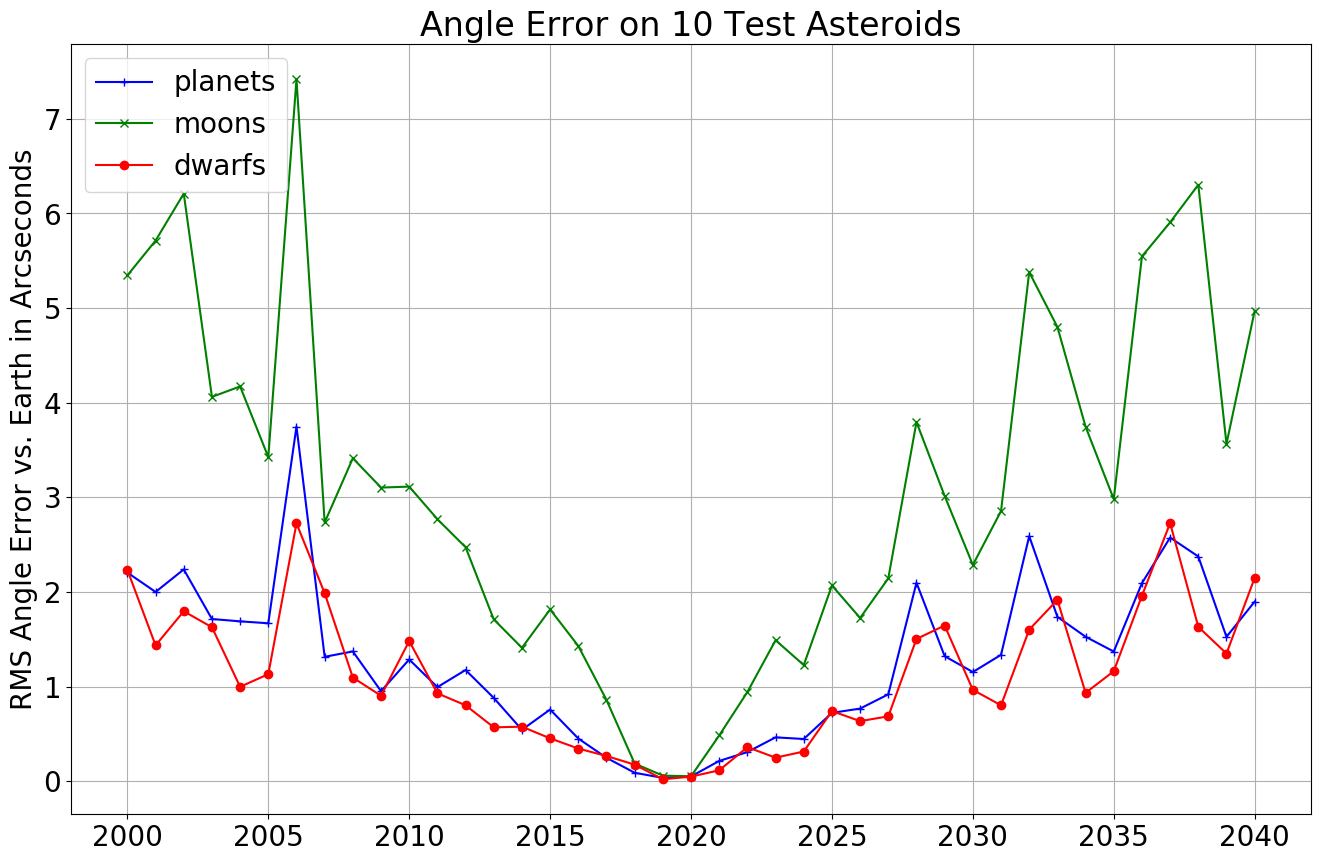
\includegraphics[width=1.0\textwidth]{sim_pos_error_comp.png}
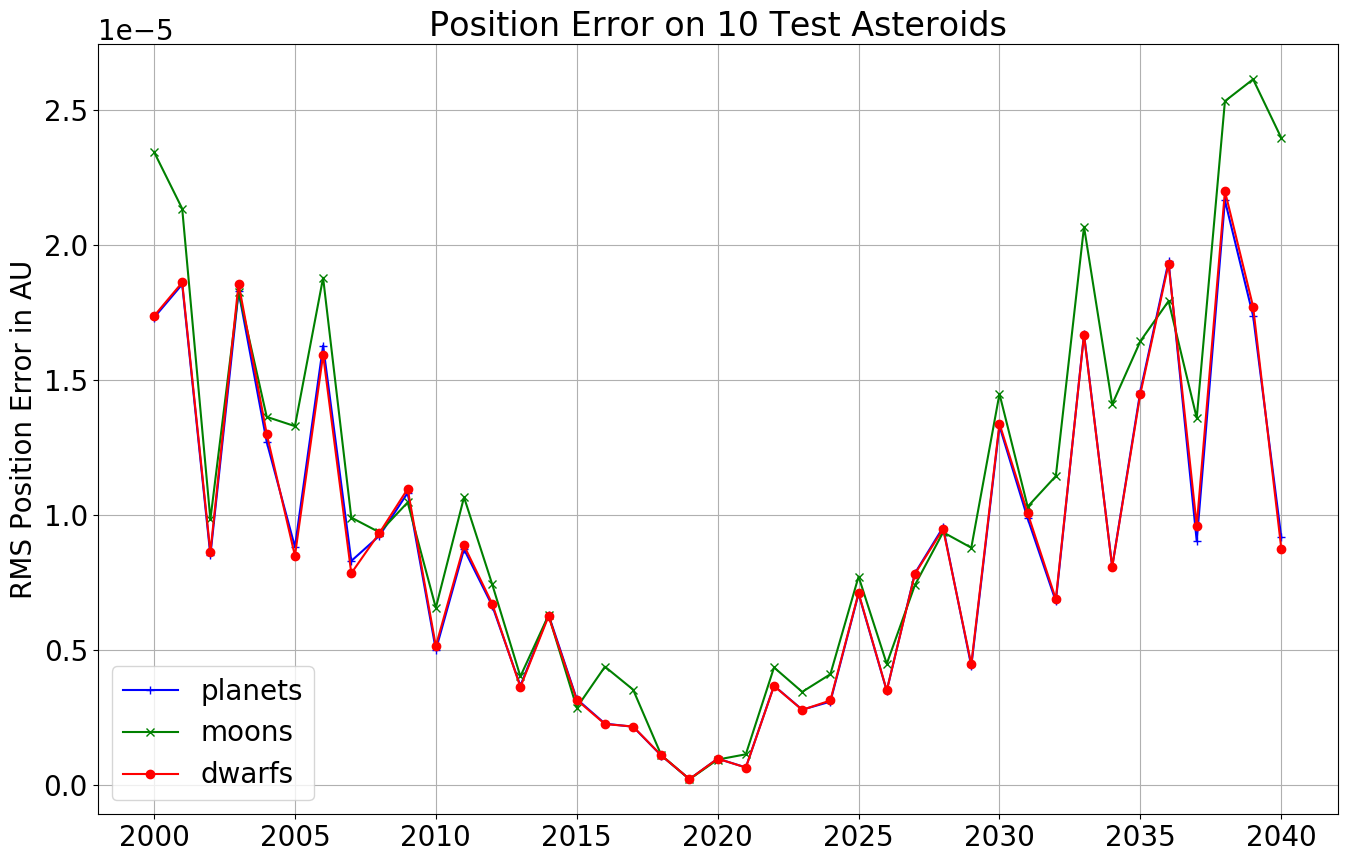
\includegraphics[width=1.0\textwidth]{sim_ang_error_comp.png}
\caption{Position and Angle Error of 10 Test Asteroids. \\
My integration is compared to positions extracted from Horizons at 40 dates from from 2000 to 2040.}
\end{center}
\end{figure}
If we focus on a plausible window of $\pm 5$ years around 2020, we can see that the selected planets integration is extremely accurate.
Angular errors 5 years out are on the order of $0.5$ arc seconds.

\section{Efficient Integration of All Known Asteroids}
\label{section_integrate_known_asteroids}

\section{Integration of Kepler Two Body Problem in Tensorflow}
\label{section_kepler_two_body_tensorflow}
